The filter design process is documented in this section including test and optimization. As stated in section \ref{sec:filtervalg} a FIR filter of type I, designed by the Kaiser window is wanted.
\subsection{Specifications}\label{sec:FIRspec} 
By the aim of letting a limited frequency band though the filter - as found in the frequency analysis chapter \ref{ch9} - the filter is to be designed as a bandpass filter. It is essential to note that the filter to be design in this project is not an adaptive filter. Meaning that the filter specification will be chosen on behalf of a specific signal includning a known noise signal. During test the filter is adapted to other signals only by chancing the specifications for the cut off frequencies.\\
This filter is determined to remove noise in the form of background speaking from a signal representing a low E note. \\
Due to the frequency analysis of single tones section \ref{sec:single} the energy in the signal is located within a frequency band from 75 Hz to 1000 Hz.  
By letting the cut off frequencies of the filter be respectively 75 Hz and 1000 Hz this makes the passband of the filter. Note that the cut off frequencies is given in $[Hz]$ instead of $[rad./sec.]$. To convert between the two the frequencies has to be relative to the sampling frequency $f_s$ such that $f_s = 2\pi$. Thus the normalized frequency transition $f_t$ is defined relative to the sampling frequency as
\begin{align}
f_t = \frac{\textit{Cut off frequency}}{\textit{Sampling frequency}}
\end{align}
\trine{Something about the analysis of the noise, maybe}

The peak approximation error $\delta_1$\trine{bør delta være forskellige?} is determined as $\delta_1=0.05$. Further the width of the transition band is determined by another $\delta_2$ as $\Delta \omega = ((f_t + \delta_2)-(f_t - \delta_2))2\pi= 0.05$.\\
The magnitude response of the ideal filter is sketched in figure \ref{fig:spec_Hd}, along with the boundaries for the real filter, provided by the defined specifications.      

\begin{figure}[H]
\centering
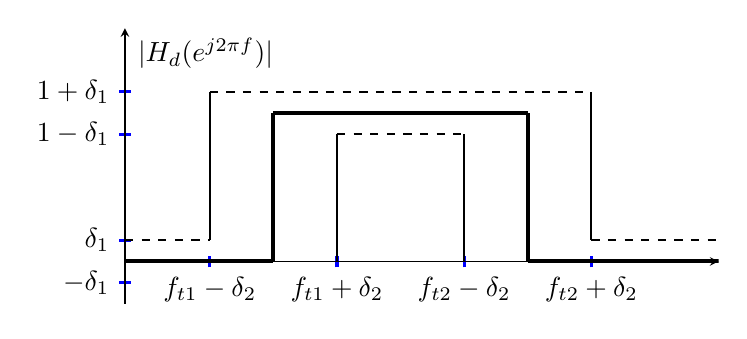
\begin{tikzpicture}[scale=1]
\begin{axis}[every tick/.style={blue, very thick}, 
scale=1.1,
unit vector ratio*=1 1 1,
axis lines = middle,
xtick={2,5,8,11},
xticklabels={$f_{t1}-\delta_2$,$f_{t1}+\delta_2$,$f_{t2}-\delta_2$,$f_{t2}+\delta_2$},
ytick={-0.5,0.5,3,4},
yticklabels={$-\delta_1$,$\delta_1$,$1-\delta_1$,$1+\delta_1$},
xmin=0,
xmax=14,
ymin=-1,
ymax=5.5]
\node at (axis cs:1.9,4.9) {$|H_d(e^{j 2\pi f})|$};
\draw[line width=0.5mm](axis cs:0,0)--(axis cs:3.5,0);
\draw[line width=0.5mm](axis cs:3.5,0)--(axis cs:3.5,3.5);
\draw[line width=0.5mm](axis cs:3.5,3.5)--(axis cs:9.5,3.5);
\draw[line width=0.5mm](axis cs:9.5,3.5)--(axis cs:9.5,0);
\draw[line width=0.5mm](axis cs:9.5,0)--(axis cs:14,0);
\draw[line width=0.25mm, dashed](axis cs:0,0.5)--(axis cs:2,0.5);
\draw[line width=0.25mm, dashed](axis cs:11,0.5)--(axis cs:14,0.5);
\draw[line width=0.25mm, dashed](axis cs:5,3)--(axis cs:8,3);
\draw[line width=0.25mm, dashed](axis cs:2,4)--(axis cs:11,4);
\draw[line width=0.25mm](axis cs:2,0.5)--(axis cs:2,4);
\draw[line width=0.25mm](axis cs:5,0)--(axis cs:5,3);
\draw[line width=0.25mm](axis cs:8,0)--(axis cs:8,3);
\draw[line width=0.25mm](axis cs:11,4)--(axis cs:11,0.5);
%\draw[line width=0.5mm](axis cs:4,0.5)--(axis cs:7,0.5);
%\node at (axis cs:1,1.5) {Passband};
%\node at (axis cs:3,1.5) {Transition};
%\node at (axis cs:5.0,1.5) {Stopband};
\end{axis}
\end{tikzpicture}
\caption{Ideal magnitude response of filter within the boundaries for the magnitude response of the final filter, given by the defined specifications.}
\label{fig:spec_Hd}
\end{figure}

Due to the method of the Kaiser window, section \ref{subsec:FIR}, the shape parameter $\beta$ and the order of the filter $M$ is determined, on behalf of $A=-20\log_{10}(\delta_1) \approx 26 $, as  
\begin{align}
\beta =& \ 0.5824(26-21)^{0.4} + 0.07886(26-21)  \approx 1.5 \\
M =& \ \frac{26-8}{2.285 \cdot 0.05\cdot 2\pi}\approx 26 
\end{align}
Note that $M$ is rounded up to nearest even integer 
\subsection{Implementation}
The implementation of the filter basically follows algorithm \ref{alg:FIR}. First filter specifications are defined. Then one function defines the ideal impulse response as the inverse Fourier transformation of the ideal filter specified on figure \ref{fig:spec_Hd}. For derivation of the ideal impulse response of a bandpass filter consult appendix \ref{appC}. Another function defines the Kaiser window from the given inputs $\beta$ and $M$. Then the filter is defined by multiplying the ideal impulse response and the Kaiser window to get a realizable impulse response. By FFT the frequency response of the filter is obtained. Figure \ref{??} illustrate a plot of the magnitude response corresponding to the filter in the frequency domain.   

\begin{algorithm}[H]
\caption{Compute type I FIR filter}
\label{alg:FIR}
\begin{algorithmic}[1] 
\State $f_s= 44100$ \Comment {Sampling frequency}
\State $M = 26$ \Comment {Order of filter} 
\State $\beta = 1.5$ \Comment {Shape parameter}
\State $N = M+1$ \Comment {Lenght of filter}
\State $f_{t1} = 75/f_s$ \Comment {Transition frequency $1$}
\State $f_{t2} = 1000/f_s$ \Comment {Transition frequency $2$}
\\
\Procedure{Compute ideal impulse response}{$h_d$}
    \For {each integer $i$ in $h_d$}
        \If {$i == \frac{M}{2}$}
        		\State $h_d[i] = 2(f_{t2} - f_{t1})$
        	\Else 
        		\State  $h_d[i] = \frac{1}{ (\pi (i - \frac{M}{2}))}(\sin(f_{t2} 2 \pi (i - \frac{M}{2})) - (\sin(f_{t1} 2 \pi (i - \frac{M}{2}))))$ 
        	\EndIf 
	\EndFor
	\State Return $h_d$
\EndProcedure
\\
\Procedure{Compute kaiser window}{$w$}
	\For {each integer $i$ in length of $N$}
		\For {each integer $j$ in length of $M$}
			\State $ sum_n = + \ (\frac{1}{j!})^2 \left( \left( \frac{\beta}{2} \sqrt{\left(1 - \left( \frac{2*i}{N-1}\right) - 1\right)^2}\right)^{2j}\right)$
			\State $ sum_d = + \ (\frac{1}{j!})^2 \left( \frac{\beta}{2}\right)^{j2}$
		\EndFor
		\State $w[i]=\frac{sum_n}{sum_d}$
	\EndFor
	\State Return $w$
\EndProcedure
\\
\Procedure{Compute frequency response}{$H$}
	\State $h = h_d \cdot w$ \Comment{Windowed impulse response}
	\State $H = fft(h)$ \Comment {Fourier transformation of impulse response}
	\State Return $H$
\EndProcedure

\end{algorithmic}
\end{algorithm}

\subsection{Validation of filter}
//////// section fra test specificationer ////////\\
To validate the filter it will be tested whether the filter fulfil the specifications that will be defined during the design process. In order to clarify the effect of the filter it will be tested on a simple known signal where a noise signal is digitally added. By this the frequency spectrum of both the pure signal and the noise is known and so is the signal to noise ratio. Hence it is possible to verify whether the filter succeed to remove the specified frequencies in order to reduce the noise. The verification will be made by analysing the frequency spectrum of the filtered signal - by plotting amplitude to frequency - compared to the original pure signal. \\
/////////////////////////////////////////////////\\
The implemented filter is to be tested according to test specifications described in section\ref{sec:testspec}. Figure \ref{??} show the frequency spectrum of the a single low E note with additive noise in form of a beat of hands clapping. Figure \ref{??} show the filtered signal.\\
/// indsæt figure ////

As described under specifications the filter is designed to remove all frequencies outside the frequency band from 75 Hz to 1000 Hz. It is seen by the figures that ...... \\
By this the filter of order ?? fulfil the specifications. Though by comparing the filtered signal with the pure music signal it seen that noise occurs in between the three significant frequencies that lays in the passband.  \\
On behalf of this test it is assumed that by changing the cut off frequencies the filter can be modified to fit other music signal.    